%\documentclass[10pt,a4paper]{article}
\documentclass[12pt,a4paper]{article}
\usepackage{graphicx,units,amsmath}
\usepackage{subfigure}
\usepackage{float}
\usepackage[ngerman, english]{babel} 
%\usepackage[utf8]{inputenc}
\setcounter{secnumdepth}{4}

\usepackage[top=2cm, bottom=2.5cm, left=3cm, right=3cm]{geometry}

%-Eingabe der Metadaten des Titelblattes--------------------------

%-Daten des Autors / Authors Data---------------------------------

\newcommand{\dcauthorpre}{~} 
\newcommand{\dcauthorsurname}{Kullmann} 
\newcommand{\dcauthorname}{Richard} 
\newcommand{\dcauthoradd}{geboren am 17.07.1996 in Berlin-Pankow}

%-Titel und Untertitel / Title and subtitle-----------------------

\newcommand{\dctitle}{Giant Diffusion in two-dimensional Neuron Models} 
\newcommand{\dcsubtitle}{~}  
% Falls dcsubtitle NICHT verwendet werden soll, {\dcsubtitle}{~} eingeben.

%-Eingabe der Betreuuernahmen / Names of the consultants---------

\newcommand{\dcconsulta}{~} 
\newcommand{\dcconsultb}{~} 
\newcommand{\dcconsultc}{~} 

%-Eingabe der Gutachternamen / Names of the approvals-------------

\newcommand{\dcapprovala}{Prof. Dr. Benjamin Lindner} 
\newcommand{\dcapprovalb}{Prof. Dr. Igor Sokolov} 
\newcommand{\dcapprovalc}{~} 

%-Information zur Universitaet------------------------------------

\newcommand{\dcdegree}{Master of Science\\(M. Sc.)} 
\newcommand{\dcsubject}{Physik} 
\newcommand{\dcfaculty}{Mathematisch-Naturwissenschaftlichen Fakult\"at I}
\newcommand{\dcinstitute}{Institut f\"ur Physik}
\newcommand{\dcuniversity}{Humboldt-Universit\"at zu Berlin}
\newcommand{\dcdean}{Prof. Dr. sc. Heinz  M\"uller}
\newcommand{\dcpresident}{Prof. Dr. Dr. h.c. Wilhelm Schulz}

%-Pruefungsdaten: eingereicht und mdl. Pruefung-------------------
%-data of submission and oral exam--------------------------------

\newcommand{\dcdatesubmitted}{5. Juni 2020} %auch wenn nicht auf dem 
%Titelblatt, bitte erf�llen!
\newcommand{\dcdateexam}{2. Juli 1999} 


% Folgende Zeile bitte nicht aendern!
\newcommand{\dckeywordsde}{\vfill \raggedright {\textbf{Schlagw\"orter:}}\\ \dckeydea, \dckeydeb, \dckeydec, \dckeyded \\}

%-englische Schlagwoerter / english keywords----------------------

\newcommand{\dckeyena}{Giant Diffusion}
\newcommand{\dckeyenb}{Two-Dimensional Neuron Models}
\newcommand{\dckeyenc}{Bistability}
\newcommand{\dckeyend}{Signal-to-Noise Ratio}

% Folgende Zeile bitte nicht aendern!
\newcommand{\dckeywordsen}{\vfill \raggedright {\textbf{Keywords:}}\\ \dckeyena, \dckeyenb, \dckeyenc, \dckeyend \\}

\newcommand{\dcpdfsubject}{Dissertation}  
\graphicspath{{images/}}
\begin{document}


%\title{Masterarbeit}
%\author{Richard Kullmann}
%\date{15.07.2019}

%----------Generierung der Titelseite-----bitte nicht ver�ndern!--------------------


\author{von \\ \dcauthorpre\ \dcauthorname\ \dcauthorsurname\ \\ \dcauthoradd}

%----------
\title{ \vspace{-2cm}\dctitle \\ 
\vspace{0.5cm}
\large{\dcsubtitle} \\ 
\vspace{0.5cm} {\Large{MASTERARBEIT}}\\ 
\vspace{0.5cm} \large{zur Erlangung des akademischen Grades \\ 
\dcdegree\\ im Fach \dcsubject \\\vspace{0.5cm}

\includegraphics[width=6cm]{husiegel}\\ 
\vspace{0.5cm} eingereicht an der \\ 
\dcfaculty \\ 
\dcinstitute\\
\dcuniversity \\}}
%-----------------
\date{\vspace{2.5cm}
%\raggedright{
%Pr\"asident der Humboldt-Universit\"at zu Berlin:\\
%\dcpresident \vspace{-0.3cm}
%}\vspace{0.5cm}\\
%
%\raggedright{
%Dekan der \dcfaculty:\\
%\dcdean \vspace{-0.3cm}
%}\vspace{0.5cm}\\
%
% auskommentiert weil nicht standard
\raggedright{
Gutachter:
\begin{enumerate} 
\item{\it\dcapprovala} \vspace{-0.3cm}
\item{\it\dcapprovalb} \vspace{-0.3cm}
%\item{\it\dcapprovalc} \vspace{-0.3cm}
\end{enumerate}} \vspace{0.5cm}
%\raggedright{
%Betreuung:
%\begin{enumerate} 
%\item{\it\dcconsulta} \vspace{-0.2cm}
%\item{\it\dcconsultb} \vspace{-0.2cm}
%\end{enumerate}} \vspace{0.5cm}
%-----------------
\raggedright{
\begin{tabular}{lll}
eingereicht am: &  &\it\dcdatesubmitted\\ % wenn nicht in der Pr�fungsordnung, die Zeile bitte auskommentieren
%Tag der m\"undlichen Pr\"ufung: & & \dcdateexam
\end{tabular}}\\ 
}
%------------------------------------- 

\maketitle

\thispagestyle{empty}
%\setcounter{page}{2}
\newpage
%-englische-Zusammenfassung---------------------------------------

%\selectlanguage{english}

%\begin{abstract}
%\setcounter{page}{2} % Nach Bedarf anpassen!
%Here is the english abstract.\\
% hier werden die englische Schlagw�rter aus Metadaten �bernommen
%\dckeywordsen				
%\end{abstract}

%-deutsche Zusammenfassung----------------------------------------

%\selectlanguage{german}

\begin{abstract}
\setcounter{page}{2} % Nach Bedarf anpassen!
The emerging field of magnetometry based on NV centers opens a variety of new experimental perspectives, including the imaging of single nuclear spins on the nanoscale. However, in order to achieve exceptionally long NV electron spin coherence times and high sensitivities, the NV spin needs to be decoupled from unwanted interactions with the environment. This can be accomplished with dynamical decoupling sequences.
\\
During the work for this thesis, multiple dynamical decoupling protocols were implemented and tested on NV centers in bulk diamond and nanodiamond. 
\\
The theoretical part covers general NV properties before treating the behaviour of a free electron spin and finally applying this on the NV center. Then, the effect of different decoupling protocols are discussed. After that, the structure and concept of the setup will be explained. In the final part, the measurements will be presented. The execution of the decoupling sequences will be demonstrated and the data will be used to extract the spectral density function of the environment.
\\
It was shown that all implemented dynamical decoupling sequences could enhance the coherence time. It was demonstrated that CPMG outperforms the other sequences on the given setup, achieving an improvement of up to a factor of 200 in the bulk diamond and 50 in nanodiamond. Finally, the examination of the spectral density functions of the spin bath gave a deeper insight in its coupling strength to the NV and its internal dynamics.\\
In the future, the limitations of the sequences will be further explored and other decoupling protocols will be tested. In addition to that, a better time and phase control has to be accomplished. These efforts will eventually lead to sensitivities high enough to detect small spin ensembles and even single molecular spins.
% hier werden die deutsche Schlagw�rter aus Metadaten �bernommen
%\dckeywordsde
\end{abstract}
\thispagestyle{empty}

\tableofcontents
\thispagestyle{empty}
\newpage
\pagenumbering{arabic}

\section{Introduction}

The human brain is one of the most investigated but still least understood subjects in scientific research. This comes as no surprise considering the huge variety of tasks it can perform efficiently and seemingly effortlessly: it constantly combines multiple sensory impressions and filters the most relevant of them to form a coherent image of the surroundings, it remembers information it has learned decades ago, it can produce the most complex thoughts and keep a whole organism working properly in the meantime. And despite the mayor improvement of processor performance and increasing interest in machine learning and artificial neural networks during the past couple of years, no technological implementation has even remotely managed to match the capability of the human brain.\\
The basis for its high functionality lies in the huge number of neurons - around 100 Billions\cite{eqnum} - and their interconnectivity: neural cells usually receive inputs from more than 10.000 other neurons\cite{izi}. Thus, in order to be able to understand how the brain works and possibly derive future applications from that, it is crucial to examine neural cells and study their characteristics. \\
Neural cells display a plethora of responses to their synaptic inputs. In general, neural activity can be divided into four mayor regimes: resting state, sub-threshold oscillations, spiking and bursting\cite{dnb}. This work will focus on bursting neurons. These exhibit phases of repetitive spiking followed by periods of quiescence. A comparable behaviour was observed for Brownian Particles underlying bistable velocity dynamics\cite{abp}\cite{bpp}, induced either via a velocity potential or movement in a biased cosine potential. In these systems, a specific range of parameters leads to diverging diffusion coefficients for vanishing noise intensity. This phenomenon is called \glqq Giant Diffusion \grqq. Applying this observation to neural cells, this could mean a large enhancement of the Signal-to-Noise Ratio through just a slight change in the system parameters. The goal of this thesis is to find out whether Giant Diffusion can be observed in a simple two-dimensional neuron model and which consequences this might have on the signal transmission, e.g. the Signal-to-Noise Ratio when the system is subject to an external stimulus.

\section{Theory}
\subsection{Quantities of interest}
In the context of Brownian Motion, there are two characteristic quantities: the ensemble of particles moves with a mean velocity
\begin{equation}
\left\langle v\right\rangle =\lim_{t\rightarrow\infty}\frac{\left\langle x(t)-x(0) \right\rangle}{t}
\end{equation}
and is subject to a diffusive spread around this average flow that can be described by the effective diffusion coefficient
\begin{equation}
D_{eff}=\lim_{t\rightarrow\infty}\frac{\left\langle x^2(t) \right\rangle-\left\langle x(t)\right\rangle ^2}{2t}
\end{equation}
\subsection{Giant Diffusion}
The term \glqq Giant Diffusion \grqq is short for \textit{Giant Enhancement of (thermal) diffusion} which was first observed around the turn of the millennium for Brownian Particles in a tilted periodic potential\cite{td}\cite{ga}\cite{dit}\cite{gd}. In general, these particles exhibit two stable velocity states. They can be \glqq trapped\grqq in a potential minimum - this is referred to as the \textit{locked state} - or they can be in the \textit{running state}. A particle gets into the running state if it has managed to overcome a hill and the frictional loss is low enough so that it is able to pass the adjacent hills as well. In the case of large friction or a strongly tilted potential, however, only one of these two states is present. If the potential is tilted in such a way that both states exist and the probabilities to be in either state are similar, many switchings between the states will occur. In the weak-noise-limit, half of the particles will be mainly in the locked state, while for the others the running state prevails. This behavior leads to diverging diffusion coefficients known as Giant Diffusion.
\subsection{Giant diffusion of Brownian Particles}
First observed by the botanist Robert Brown in 1828\cite{bm}, the term \textit{Brownian Motion} describes the irregular movement of particles in a viscous medium, whose apparently random changes of direction are caused by collisions with smaller particles or molecules.
\\
Ordinary Brownian Motion obeys a simple linear Langevin-equation:
\begin{align*}
\text{m}\dot{v}=-\lambda v+\xi(t)
\end{align*}
The evolution of the velocity $v$ of the particle is affected by a linear friction term with coefficient $\lambda$ and a random force $\xi(t)$. \\
\\ 
In the following, two different systems with Brownian Motion dynamics exhibiting Giant Diffusion are presented. These were the motivation for my research on bursting neuron models.
\subsubsection{Active Brownian Particles}
Active Brownian Motion can be observed on small organisms, like bacteria or cells, which are able to move on their own. In order to model the behaviour of such an object, a more general friction term needs to be introduced into the Langevin-equation:
\begin{align*}
\dot{v}=-f(v)+\xi(t)
\end{align*}
Here, the noise was assumed to be additive and the mass was omitted due to clarity.
An accurate description of the self-propulsion can be accomplished by choosing the function $f$ in such a way that it attains negative values at small velocities and becomes greater than zero at large speed. Thus, at small velocities the particle will accelerate and with increasing velocity, regular friction will start to affect its motion.
\\
A system like this was studied by Lindner and Nicola in 2008\cite{abp}. They chose a cubic function for the friction term, $f(v)=v-v^3+F$, allowing them to write the equation of motion in terms of a quartic velocity potential $U(v)$:
\begin{equation}
\dot{v}=-U'(v)+\xi(t)
\end{equation}
with $U(v)=\frac{1}{4}v^4-\frac{1}{2}v^2-Fv$.
\begin{figure}[H]
	\centering
	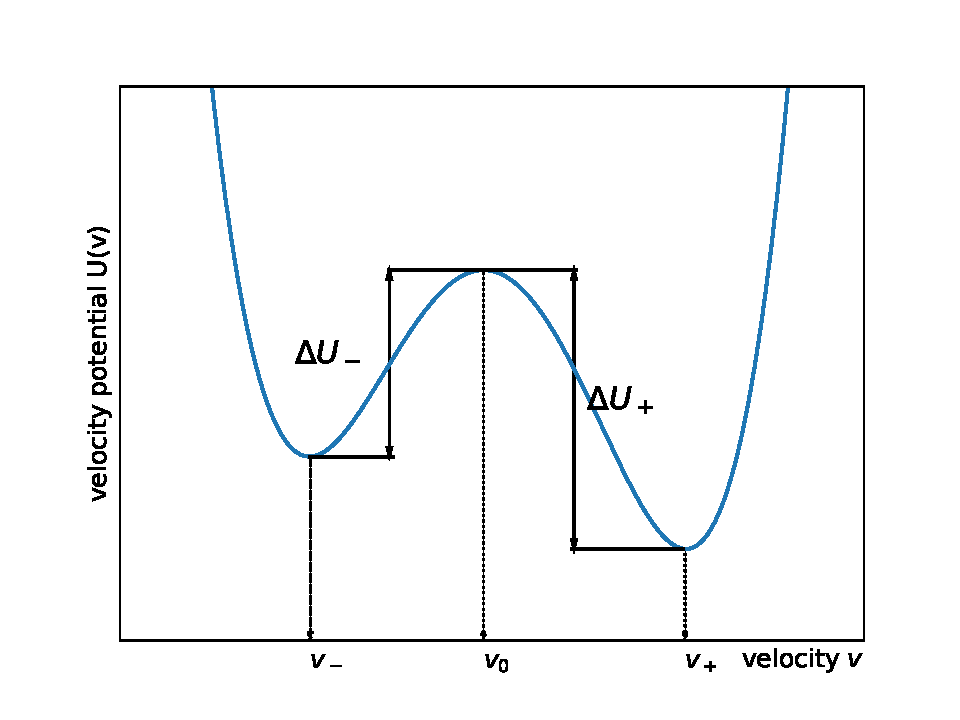
\includegraphics[scale=1]{velpot.pdf} 
	\caption{tilted velocity potential of an Active Brownian Particle}
	\label{velpot}
\end{figure}
This potential shows two minima at $v_\pm$, representing the stable velocity states \glqq forwards\grqq and \glqq backwards\grqq, and a maximum at $v_0$. In order to transition from $v_\pm$ into the other state, the particle needs to overcome a barrier of height $\Delta U\pm$.  
\\
Their simulations revealed a certain region of bias forces $F$, in which giant diffusion occurred.
\begin{figure}[H]
	\centering
	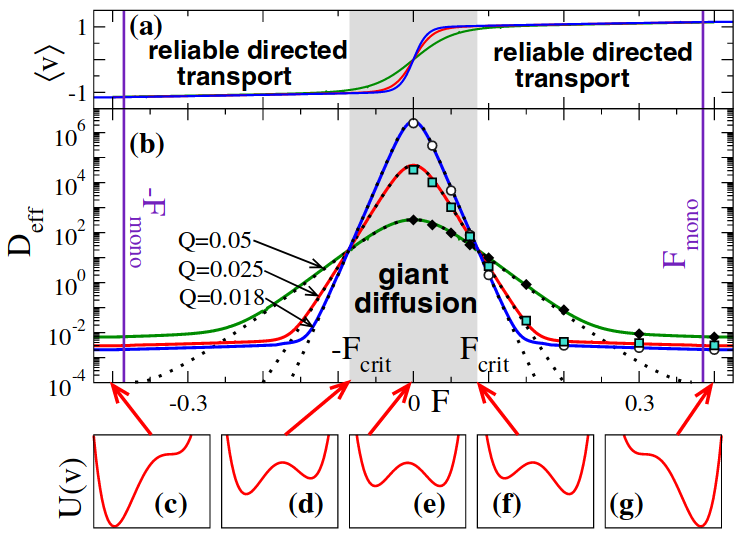
\includegraphics[scale=0.5]{mess08.png}\caption{Simulation of velocity and effective diffusion coefficient for Active Brownian Particles underlying a tilted velocity potential,taken from \cite{abp}}
	\label{abpsim}
\end{figure}
Inside this region, the diffusion coefficients increase with decreasing noise intensity, while they decrease outside of this region. In other words, in the weak noise limit, the diffusion coefficients diverge in the critical region and vanish outside of it. The critical force lies at the border of this region and emerges from the intersection points of the diffusion coefficients for different noise levels. A simple criterion could be found for these intersection points: at the critical force, one potential barrier is twice as high as the other potential barrier. 
Furthermore, it is remarkable that the reliable directed transport which takes place outside of the critical region appears much earlier than the monostability of the velocity potential, which is a obviously only a primitive criterion for reliable transport in one direction. 
The mean velocity displays a more regular behavior. It is almost constant at a value less than zero up to small negative forces, then undergoes a sharp increase to a positive value and barely changes afterwards. They intersect as well, approximately at the position where the diffusion coefficient gets maximal.
\subsubsection{Regular Brownian Particles in a tilted periodic potential}
On their own, ordinary Brownian Particles do not exhibit bistable velocity dynamics which may lead to giant diffusion. But as mentioned before, this can be done by adding a periodic potential to the equation of motion:
\begin{equation}
\dot{v}=-\gamma v-U'(x)+\sqrt{2\gamma kT}\xi(t)
\end{equation}
with $U(x)=-Fx-d\cos(x)$. This system was discussed with respect to giant diffusion in a paper by Lindner and Sokolov from 2016\cite{bpp}. Now, in contrast to the Active Brownian Particle, the evolution of the system is not governed by a velocity potential, but by a spatial potential:
\begin{figure}[H]
	\subfigure[]{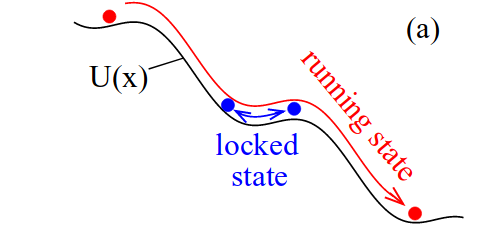
\includegraphics[width=0.5\textwidth]{veldynupper.png}} 
	\subfigure[]{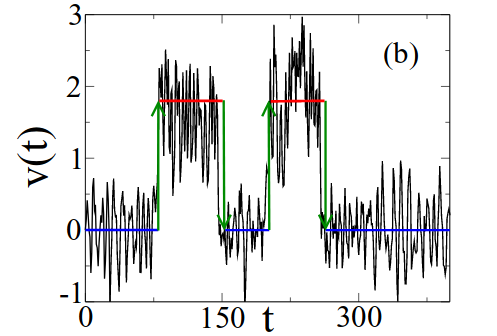
\includegraphics[width=0.5\textwidth]{veldynlower.png}} 
	\caption{Figure (a) visualizes the motion of a Brownian Particle in a periodic potential, on the right one can see the bistable velocity dynamics. The oscillations thereby arise from local extrema of the potential.}
	\label{veldyn} 
\end{figure}
Also for the Brownian Particles in a cosine potential, there was a finite range of bias forces, for which giant diffusion could be observed:
\begin{figure}[H]
	\centering
	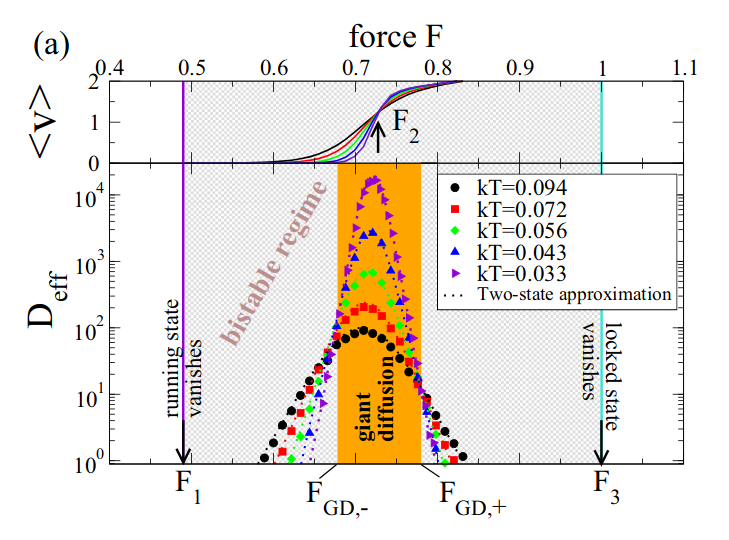
\includegraphics[scale=0.5]{nbpsim1.png}\caption{Simulation of velocity and effective diffusion coefficient for Brownian Particles in a tilted periodic potential,taken from \cite{bpp}}
	\label{anbpsim}
\end{figure}
Again, all curves of the diffusion coefficient intersect at two points and diverge in between those points for decreasing noise intensities while going to zero on the outside and the velocity curves intersect approximately at the maximum of the diffusion coefficient. And also here the region of giant diffusion is much smaller than the range of bias forces, where both states coexist. Two other variables that help characterize the system are the transition rates between the states, that is from the locked to the running state and vice versa. Even though there were no actual potential barriers present, these turned out to obey an Arrhenius or Kramers law, respectively, as can be seen from an Arrhenius plot:
\begin{figure}[H]
	\centering
	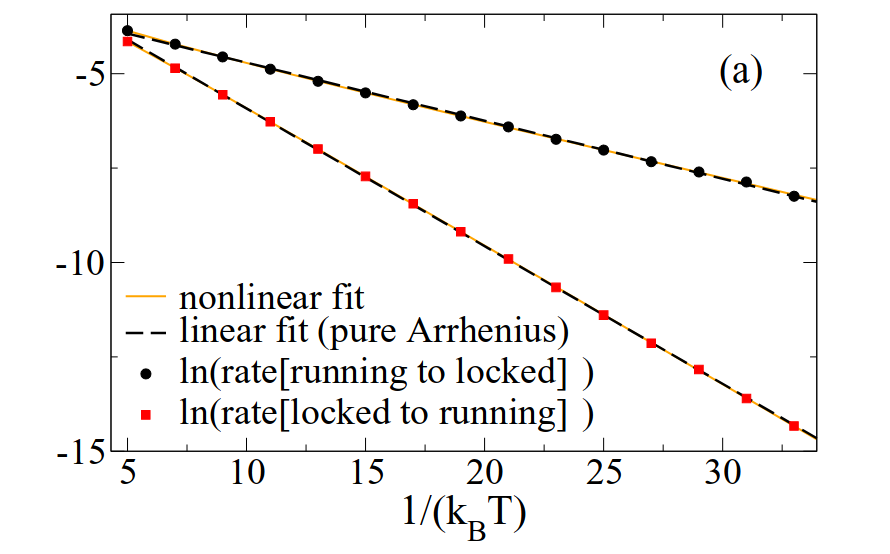
\includegraphics[scale=0.5]{kramerfit.png}\caption{Fits of the transition rates with both an Arrhenius and a Kramers law, taken from \cite{bpp}}
	\label{bparr}
\end{figure}
In this example, the Arrhenius fit as well as the Kramers fit yield good agreements with the data. From these fits one can extract effective potential barriers. The relation found for the potential barriers of the Active Brownian Particle can be tested by plotting the effective barriers and their double value:
\begin{figure}	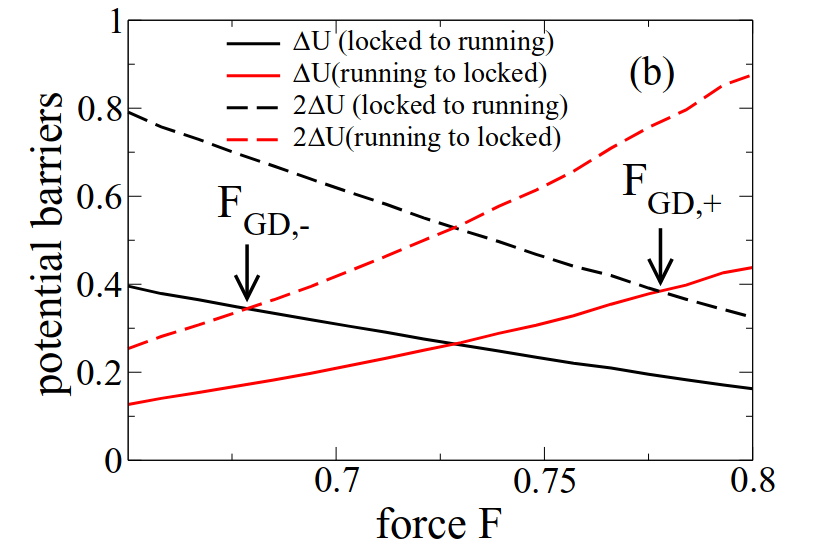
\includegraphics[scale=0.25]{barrierplot.png}\
\end{figure}
\bibliography{quellen}
\bibliographystyle{ieeetr}
\section*{Selbst\"andigkeitserkl\"arung}


Ich erkl\"are hiermit, dass ich die vorliegende Arbeit selbst\"andig verfasst und 
noch nicht f\"ur andere Pr\"ufungen eingereicht habe. S\"amtliche Quellen 
einschlie\ss lich Internetquellen, die unver\"andert oder abgewandelt wiedergegeben 
werden, insbesondere Quellen f\"ur Texte, Grafiken, Tabellen und Bilder, sind als 
solche kenntlich gemacht. Mir ist bekannt, dass bei Verst\"o\ss en gegen diese 
Grunds\"atze ein Verfahren wegen T\"auschungsversuchs bzw. T\"auschung eingeleitet 
wird.\\[3cm]
%
\includegraphics{unterschrift_richard}\\ 
Berlin, \dcdatesubmitted
\end{document}

